% Provenance (never printed): cycle 3 "La planete Terre. Les etres vivants
% dans leur environnement" (natural phenomena: volcanoes and earthquakes,
% natural hazards and the behaviour to adopt); see sources/book1/PROVENANCE.md.
% Book 1, grade 4, chapter 2.
\chapter{Vulkanen en aardbevingen: een eerste blik}\label{ch:g4:volcanoes-earthquakes-first-look}

Op maandagavond toont het journaal een \omterm{def:g4:volcanoes-earthquakes-first-look:volcano}{vulkaan} op een eiland ver weg. In
het donker spuit een fontein van gloeiend oranje \omterm{def:g3:stones-pebbles-sand:rock}{gesteente} uit een spleet
in de grond, en \omterm{def:g1:landscapes-around-us:water}{rivieren} van vuur stromen langzaam de helling af naar de
\omterm{def:g2:water-on-earth:ocean}{zee}, sissend en dampend. Op donderdag toont het journaal een andere plek:
een stadje waar bij zonsopgang de grond een halve minuut lang schudde.
Schoorstenen vielen op straat, en een oud huis schoof van zijn fundering.

Twee heel verschillende gebeurtenissen. Toch komen ze allebei van diep in
de Aarde, en, zoals we zullen zien, ze gebeuren allebei veel vaker in
sommige delen van de wereld dan in andere.

\begin{recall}
\omterm{def:g1:landscapes-around-us:landform}{Bergen}, \omterm{def:g1:landscapes-around-us:landform}{heuvels}, \omterm{def:g1:landscapes-around-us:landform}{dalen} en \omterm{def:g1:landscapes-around-us:landform}{vlakten} zijn de vormen van het land
(\cref{ch:g1:landscapes-around-us}). Het land van de Aarde ligt in zeven
\omterm{def:g3:continents-and-oceans:continent}{continenten}, tussen vijf \omterm{def:g2:water-on-earth:ocean}{oceanen}; de Stille \omterm{def:g2:water-on-earth:ocean}{Oceaan} is de grootste \omterm{def:g2:water-on-earth:ocean}{oceaan}
(\cref{ch:g3:continents-and-oceans}).
\end{recall}

\section{Een vulkaan barst uit}

Diep onder onze voeten is de Aarde heel heet. Op sommige plaatsen is het
\omterm{def:g3:stones-pebbles-sand:rock}{gesteente} daar zo heet dat het gesmolten is. Dit gesmolten \omterm{def:g3:stones-pebbles-sand:rock}{gesteente} is
lichter dan het \omterm{def:g3:stones-pebbles-sand:rock}{vaste gesteente} eromheen, dus stijgt het langzaam op, zoals
een kurk in water. Waar het een weg naar buiten vindt, ontstaat een \omterm{def:g4:volcanoes-earthquakes-first-look:volcano}{vulkaan}.

\begin{definition}[Vulkaan]\label{def:g4:volcanoes-earthquakes-first-look:volcano}
Een \emph{vulkaan}\index{vulkaan} is een plek waar gesmolten \omterm{def:g3:stones-pebbles-sand:rock}{gesteente} van
diep in de Aarde aan het oppervlak komt, en ook de \omterm{def:g1:landscapes-around-us:landform}{heuvel} of \omterm{def:g1:landscapes-around-us:landform}{berg} die het
gesmolten \omterm{def:g3:stones-pebbles-sand:rock}{gesteente} daar laag na laag opbouwt.
\end{definition}

\begin{definition}[Uitbarsting, lava en vulkanische as]\label{def:g4:volcanoes-earthquakes-first-look:eruption}
Een \emph{uitbarsting}\index{uitbarsting} is de tijd waarin een \omterm{def:g4:volcanoes-earthquakes-first-look:volcano}{vulkaan}
gesmolten \omterm{def:g3:stones-pebbles-sand:rock}{gesteente}, as en gas uitstoot. \emph{Lava}\index{lava} is
gesmolten \omterm{def:g3:stones-pebbles-sand:rock}{gesteente} dat over het oppervlak uitvloeit; het stroomt, koelt dan
af en wordt hard tot nieuw \omterm{def:g3:stones-pebbles-sand:rock}{gesteente}.
\emph{Vulkanische as}\index{vulkanische as} bestaat uit piepkleine stukjes \omterm{def:g3:stones-pebbles-sand:rock}{gesteente} en glas die door een
uitbarsting de lucht in worden geblazen; het valt terug als een grijze
\omterm{def:g4:clouds-rain-snow:precipitation}{sneeuw}.
\end{definition}

\begin{omfigure}
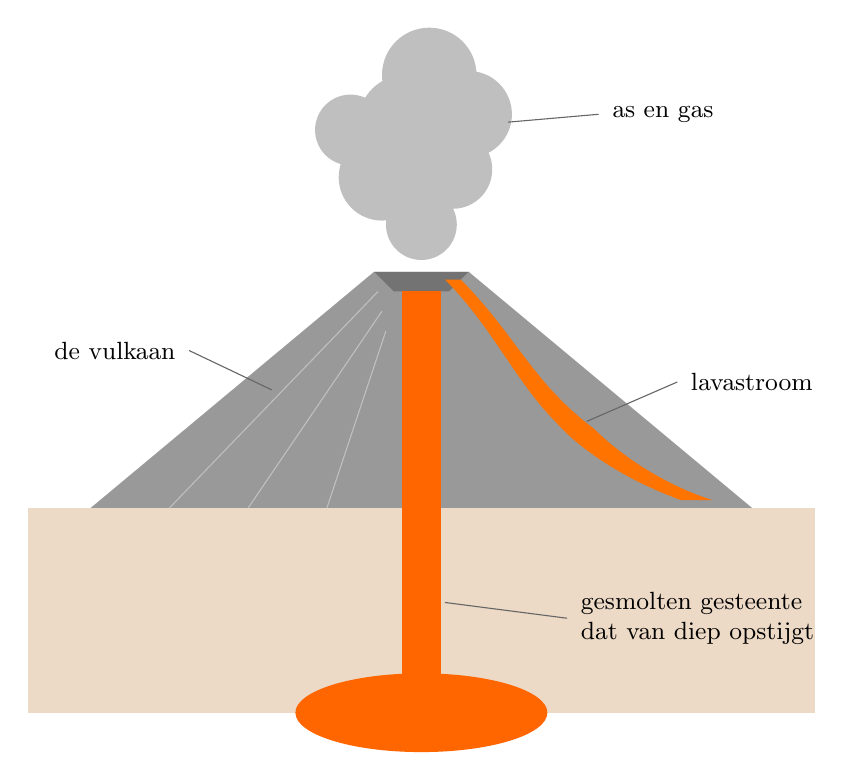
\begin{tikzpicture}[font=\small]
  % ground and deep rock
  \fill[brown!30] (-5,-2.6) rectangle (5,0);
  % the volcano
  \fill[black!40] (-4.2,0) -- (-0.6,3.0) -- (0.6,3.0) -- (4.2,0) -- cycle;
  \fill[black!55] (-0.6,3.0) -- (-0.35,2.75) -- (0.35,2.75) -- (0.6,3.0) -- cycle;
  % layers inside the cone
  \foreach \k in {1,2,3}
    \draw[black!25] (-4.2+1.0*\k,0) -- (-0.6+0.05*\k,3.0-0.25*\k);
  % molten rock rising from deep below
  \fill[orange!80!red] (-0.25,-2.6) -- (-0.25,2.75) -- (0.25,2.75) -- (0.25,-2.6) -- cycle;
  \fill[orange!80!red] (0,-2.6) ellipse (1.6 and 0.5);
  % lava flow on the right flank
  \fill[orange!90!red] (0.5,2.9) .. controls (1.2,2.2) and (1.4,1.6) .. (2.2,1.0)
    .. controls (2.6,0.6) and (3.2,0.25) .. (3.7,0.1) -- (3.3,0.1)
    .. controls (2.6,0.35) and (2.0,0.75) .. (1.7,1.1)
    .. controls (1.2,1.6) and (0.9,2.3) .. (0.3,2.9) -- cycle;
  % ash and gas cloud
  \foreach \x/\y/\r in {0/3.6/0.45, -0.5/4.2/0.55, 0.4/4.3/0.5, -0.2/4.9/0.6, 0.6/5.0/0.55, -0.9/4.8/0.45, 0.1/5.5/0.6}
    \fill[black!25] (\x,\y) circle (\r);
  % labels
  \node[anchor=west] at (2.3,5.0) {as en gas};
  \draw[black!60] (2.25,5.0) -- (1.1,4.9);
  \node[anchor=west] at (3.3,1.6) {lavastroom};
  \draw[black!60] (3.25,1.6) -- (2.1,1.1);
  \node[anchor=east] at (-3.0,2.0) {de vulkaan};
  \draw[black!60] (-2.95,2.0) -- (-1.9,1.5);
  \node[anchor=west, align=left] at (1.9,-1.4) {gesmolten gesteente\\dat van diep opstijgt};
  \draw[black!60] (1.85,-1.4) -- (0.3,-1.2);
\end{tikzpicture}

{\small Een \omterm{def:g4:volcanoes-earthquakes-first-look:volcano}{vulkaan} die uitbarst (getekend, niet op schaal). Gesmolten
\omterm{def:g3:stones-pebbles-sand:rock}{gesteente} stijgt van diep beneden op en komt bovenaan naar buiten: het
stroomt naar beneden als \omterm{def:g4:volcanoes-earthquakes-first-look:eruption}{lava}, terwijl as en gas hoog de lucht in worden
geblazen. Elke \omterm{def:g4:volcanoes-earthquakes-first-look:eruption}{uitbarsting} voegt een nieuwe laag toe aan de \omterm{def:g1:landscapes-around-us:landform}{berg}.}
\label{fig:g4:volcanoes-earthquakes-first-look:volcano}
\end{omfigure}

Niet alle \omterm{def:g4:volcanoes-earthquakes-first-look:eruption}{uitbarstingen} zien er hetzelfde uit. Bij sommige is de \omterm{def:g4:volcanoes-earthquakes-first-look:eruption}{lava}
dun vloeibaar: ze stroomt rustig naar buiten in gloeiende \omterm{def:g1:landscapes-around-us:water}{rivieren} die
kilometers ver kunnen stromen, soms helemaal tot in \omterm{def:g2:water-on-earth:ocean}{zee}. Bij andere is het
gesmolten \omterm{def:g3:stones-pebbles-sand:rock}{gesteente} dik en vol gas, zoals een geschudde fles prik: als het
naar buiten barst, ontploft het in een enorme aszuil die hoog de lucht in
stijgt.

\begin{omfigure}
\begin{minipage}[b]{0.56\linewidth}\centering
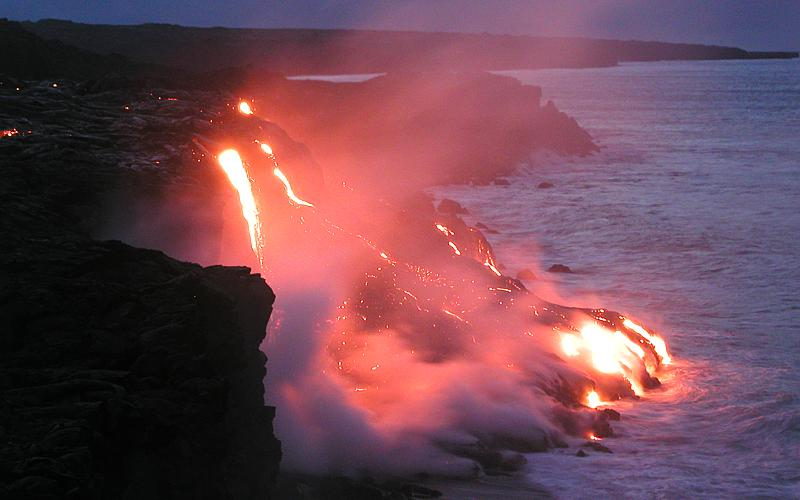
\includegraphics[width=\linewidth]{images/book1/g4-lava-ocean.jpg}

{\small Een rustige \omterm{def:g4:volcanoes-earthquakes-first-look:eruption}{uitbarsting}: \omterm{def:g4:volcanoes-earthquakes-first-look:eruption}{lava} stroomt over een klif in de \omterm{def:g2:water-on-earth:ocean}{oceaan},
op Hawaï. Foto: USGS Hawaiian Volcano Observatory (publiek domein).}
\end{minipage}\hfill
\begin{minipage}[b]{0.4\linewidth}\centering
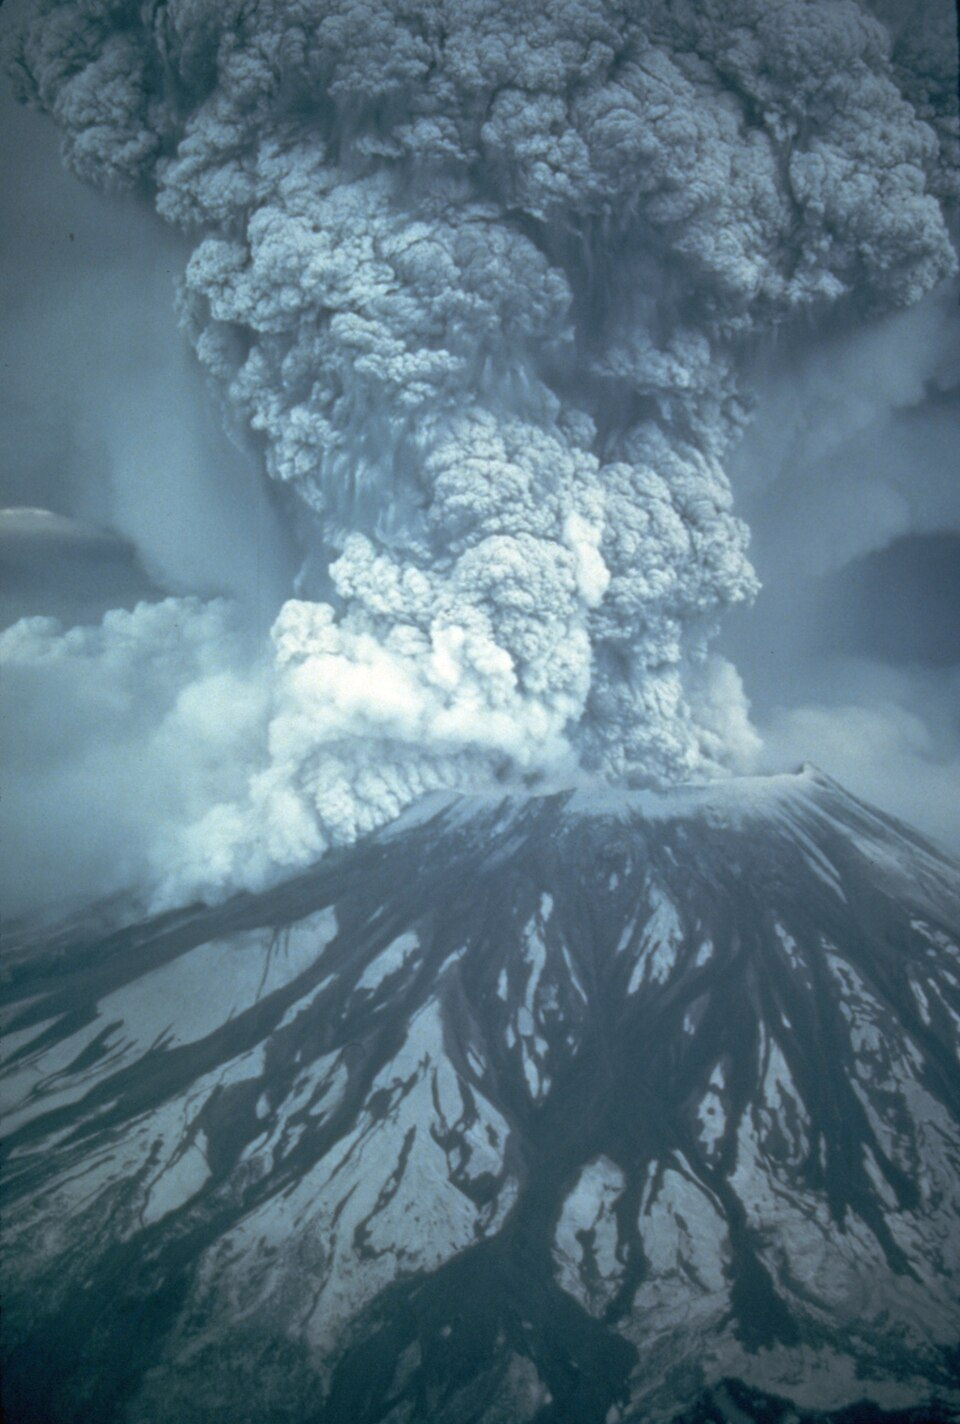
\includegraphics[width=0.78\linewidth]{images/book1/g4-st-helens.jpg}

{\small Een explosieve \omterm{def:g4:volcanoes-earthquakes-first-look:eruption}{uitbarsting}: Mount St.~Helens, Verenigde Staten,
18~mei 1980. Foto: Austin Post, USGS (publiek domein).}
\end{minipage}
% ledger: usgs:pu-oo-ocean, usgs:msh-1980
\label{fig:g4:volcanoes-earthquakes-first-look:two-eruptions}
\end{omfigure}

\begin{example}[Mount St.~Helens, 1980]\label{ex:g4:volcanoes-earthquakes-first-look:st-helens}
In het voorjaar van 1980 groeide er een bult op de flank van Mount
St.~Helens, doordat gesmolten \omterm{def:g3:stones-pebbles-sand:rock}{gesteente} in de \omterm{def:g1:landscapes-around-us:landform}{berg} naar boven drukte. Op
de ochtend van 18~mei schudde een kleine \omterm{def:g4:volcanoes-earthquakes-first-look:earthquake}{aardbeving} de \omterm{def:g1:landscapes-around-us:landform}{berg}, de bult gleed
weg in een reusachtige aardverschuiving, en de \omterm{def:g4:volcanoes-earthquakes-first-look:volcano}{vulkaan} explodeerde opzij en
naar boven. De bovenste 400~meter van de \omterm{def:g1:landscapes-around-us:landform}{berg} waren verdwenen: de top werd
een enorme krater.
% ledger: usgs:msh-1980
\end{example}

\section{De grond schudt}

Het \omterm{def:g3:stones-pebbles-sand:rock}{gesteente} diep onder onze voeten staat niet helemaal stil. Heel
langzaam wordt het geduwd en getrokken. Het buigt een beetje door, zoals
een liniaal waar je aan beide uiteinden tegen duwt --- tot het plotseling
breekt en verschuift. De schok laat de grond kilometers in de omtrek
schudden.

\begin{definition}[Aardbeving]\label{def:g4:volcanoes-earthquakes-first-look:earthquake}
Een \emph{aardbeving}\index{aardbeving} is een plotseling schudden van de
grond, veroorzaakt door \omterm{def:g3:stones-pebbles-sand:rock}{gesteente} dat diep onder de grond breekt en
verschuift.
\end{definition}

Een \omterm{def:g4:volcanoes-earthquakes-first-look:earthquake}{aardbeving} duurt meestal maar een paar seconden, bij de grootste soms
een minuut of twee. De meeste \omterm{def:g4:volcanoes-earthquakes-first-look:earthquake}{aardbevingen} zijn zo klein dat niemand ze
voelt: alleen instrumenten merken ze op. Een sterke \omterm{def:g4:volcanoes-earthquakes-first-look:earthquake}{aardbeving} kan de grond
laten golven als het dek van een schip, wegen doen scheuren en muren en
huizen laten instorten.

\begin{omfigure}
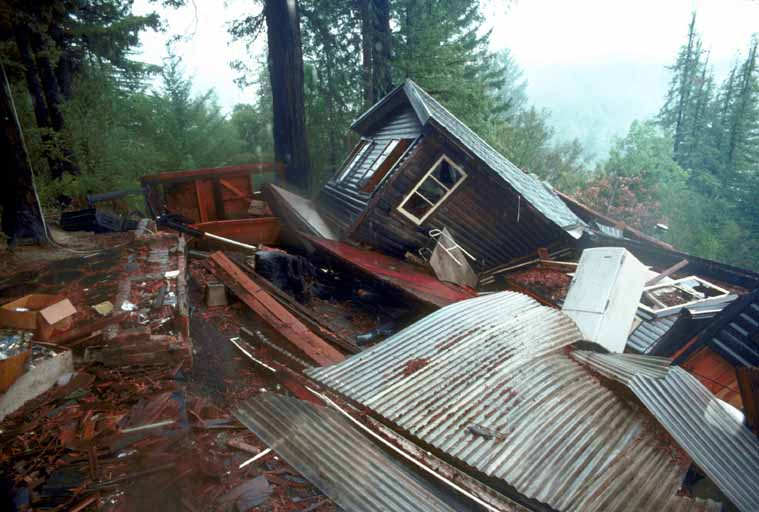
\includegraphics[width=0.55\linewidth]{images/book1/g4-loma-prieta-house.jpg}

{\small Na een sterke \omterm{def:g4:volcanoes-earthquakes-first-look:earthquake}{aardbeving} in Californië in 1989: dit houten huis
werd opzij van zijn betonnen fundering geworpen. Foto: J.~K.~Nakata, USGS
(publiek domein).}
% ledger: usgs:loma-prieta-house
\end{omfigure}

\begin{remark}[Hoe vaak?]\label{rem:g4:volcanoes-earthquakes-first-look:how-often}
Geologen houden een lijst bij van alle grote \omterm{def:g4:volcanoes-earthquakes-first-look:earthquake}{aardbevingen} op Aarde. In de
50 jaar van 1976 tot 2025 telt de lijst 7\,031 grote \omterm{def:g4:volcanoes-earthquakes-first-look:earthquake}{aardbevingen} (sterk
genoeg om gebouwen in de buurt te beschadigen): ongeveer 141 per jaar, of
bijna 3 per week. De allergrootste, die hele steden kunnen verwoesten, zijn
er ongeveer 14 per jaar. Op diezelfde Aarde zijn in de laatste
twaalfduizend jaar of zo ongeveer 1\,200 \omterm{def:g4:volcanoes-earthquakes-first-look:volcano}{vulkanen} uitgebarsten.
% ledger: data:usgs-comcat, data:gvp
\end{remark}

\section{Waar vulkanen en aardbevingen voorkomen}

Als \omterm{def:g4:volcanoes-earthquakes-first-look:volcano}{vulkanen} en \omterm{def:g4:volcanoes-earthquakes-first-look:earthquake}{aardbevingen} zomaar overal voorkwamen, zouden de stippen
gelijkmatig over een \omterm{def:g3:continents-and-oceans:world-map}{wereldkaart} verspreid liggen. Dat doen ze niet.

De \omterm{def:g2:drawing-to-map:map}{kaart} hieronder laat een opvallend patroon zien. De meeste \omterm{def:g4:volcanoes-earthquakes-first-look:volcano}{vulkanen} en
de meeste grote \omterm{def:g4:volcanoes-earthquakes-first-look:earthquake}{aardbevingen} liggen in lange, smalle gordels. De langste
van allemaal loopt rond de Stille \omterm{def:g2:water-on-earth:ocean}{Oceaan}: van Nieuw-Zeeland omhoog via
Indonesië, de Filipijnen en Japan, naar Alaska, en dan helemaal langs de
westkust van Amerika naar beneden tot de punt van Chili. Door de vele
\omterm{def:g4:volcanoes-earthquakes-first-look:volcano}{vulkanen} wordt die gordel vaak de ``Ring van Vuur'' genoemd.

\begin{example}[Tellen op de kaart]\label{ex:g4:volcanoes-earthquakes-first-look:shares}
We hebben de stippen geteld die in de gekleurde ring liggen (binnen
500~kilometer van zijn middenlijn). Van de 1\,214 \omterm{def:g4:volcanoes-earthquakes-first-look:volcano}{vulkanen} liggen er 837 in
de ring: ongeveer 2 op de 3. Van de 696 allergrootste \omterm{def:g4:volcanoes-earthquakes-first-look:earthquake}{aardbevingen} liggen
er 532 in de ring: ongeveer 3 op de 4. De ring beslaat maar een klein deel
van de Aarde, maar hij bevat de meeste \omterm{def:g4:volcanoes-earthquakes-first-look:volcano}{vulkanen} en \omterm{def:g4:volcanoes-earthquakes-first-look:earthquake}{aardbevingen}.
% ledger: data:gvp, data:usgs-comcat
\end{example}

\begin{omfigure}
\begin{tikzpicture}
\begin{axis}[ommap, width=\linewidth, xtick=\empty, ytick=\empty, grid=none,
    legend style={font=\scriptsize, at={(0.5,-0.02)}, anchor=north,
      draw=none, legend columns=3, /tikz/every even column/.append style={column sep=6pt}},
    legend cell align=left]
  \addplot[fill=omHypsLandA!85!black, draw=black!45, line width=0.2pt, forget plot]
    table {figdata/out/shared-geo-land.dat};
  \addplot[orange!80!black, opacity=0.35, line width=9pt, line cap=round, line join=round]
    table {figdata/out/grade-4-ring_of_fire-ring.dat};
  \addlegendentry{de ring rond de Stille Oceaan}
  \addplot[only marks, mark=triangle*, mark size=1.3pt, red!75!black]
    table[x=lon, y=lat] {figdata/out/grade-4-ring_of_fire-volcanoes.dat};
  \addlegendentry{een vulkaan (laatste 12\,000 jaar)}
  \addplot[only marks, mark=*, mark size=1.0pt, black, fill opacity=0.6]
    table[x=lon, y=lat] {figdata/out/grade-4-ring_of_fire-quakes7.dat};
  \addlegendentry{een allergrootste aardbeving (1976--2025)}
\end{axis}
\end{tikzpicture}

{\small \omterm{def:g4:volcanoes-earthquakes-first-look:volcano}{Vulkanen} die in de laatste twaalfduizend jaar of zo zijn
uitgebarsten, en de allergrootste \omterm{def:g4:volcanoes-earthquakes-first-look:earthquake}{aardbevingen} van 1976--2025. De meeste
liggen langs een ring van eilandketens en gebergten rond de Stille \omterm{def:g2:water-on-earth:ocean}{Oceaan}
(gekleurd). Gegevens: Smithsonian Global Volcanism Program;
aardbevingscatalogus van de U.S. Geological Survey; kustlijnen Natural
Earth.}
\label{fig:g4:volcanoes-earthquakes-first-look:map}
% ledger: data:gvp, data:usgs-comcat, data:ne-land
\end{omfigure}

Andere gordels zijn kleiner: een ervan loopt door het zuiden van Europa en
Azië, van de Middellandse \omterm{def:g2:water-on-earth:ocean}{Zee} tot de Himalaya; andere lopen midden door de
\omterm{def:g2:water-on-earth:ocean}{oceanen}, waar de \omterm{def:g4:volcanoes-earthquakes-first-look:volcano}{vulkanen} onder water verborgen liggen. Sommige plaatsen,
zoals Hawaï, hebben \omterm{def:g4:volcanoes-earthquakes-first-look:volcano}{vulkanen} ver van elke gordel. Waarom de gordels liggen
waar ze liggen, is een vraag voor \cref{ch:g7:plate-tectonics}: het antwoord
verklaart de vorm van de hele \omterm{def:g2:drawing-to-map:map}{kaart}.

\section{Veilig blijven}

Niemand kan een \omterm{def:g4:volcanoes-earthquakes-first-look:eruption}{uitbarsting} of een \omterm{def:g4:volcanoes-earthquakes-first-look:earthquake}{aardbeving} tegenhouden. Maar wie weet
wat hij moet doen, redt levens.

\begin{omfigure}
\begin{tikzpicture}[font=\small, line cap=round, line join=round]
  % --- panel 1: DROP onto hands and knees
  \begin{scope}
    \draw[black!30] (-0.2,0) -- (2.8,0);
    \fill[omDef] (0.62,0.98) circle (0.21);
    \draw[omDef, line width=2.2pt] (0.88,0.98) -- (2.0,0.95);
    \draw[omDef, line width=2pt] (0.95,0.96) -- (0.95,0.05);
    \draw[omDef, line width=2pt] (2.0,0.95) -- (1.98,0.08) -- (2.65,0.08);
    \node[font=\bfseries] at (1.3,-0.45) {BUKKEN};
    \node[font=\scriptsize, align=center] at (1.3,-0.95) {op je handen\\en knieën};
  \end{scope}
  % --- panel 2: COVER under a table
  \begin{scope}[xshift=4cm]
    \draw[black!30] (-0.2,0) -- (2.8,0);
    \fill[brown!60!black] (-0.1,1.45) rectangle (2.7,1.6);
    \draw[brown!60!black, line width=2pt] (0.1,1.45) -- (0.1,0) (2.5,1.45) -- (2.5,0);
    \fill[omDef] (0.75,0.95) circle (0.2);
    \draw[omDef, line width=2.2pt] (0.95,0.85) -- (1.95,0.8);
    \draw[omDef, line width=2pt] (1.9,0.8) -- (1.65,0.05) -- (2.25,0.05);
    \draw[omDef, line width=2pt] (1.0,0.85) -- (0.7,1.2) -- (0.5,0.95);
    \node[font=\bfseries] at (1.3,-0.45) {DEKKEN};
    \node[font=\scriptsize, align=center] at (1.3,-0.95) {je hoofd en nek,\\onder een stevige tafel};
  \end{scope}
  % --- panel 3: HOLD ON to the table leg
  \begin{scope}[xshift=8cm]
    \draw[black!30] (-0.2,0) -- (2.8,0);
    \fill[brown!60!black] (-0.1,1.45) rectangle (2.7,1.6);
    \draw[brown!60!black, line width=2pt] (0.1,1.45) -- (0.1,0) (2.5,1.45) -- (2.5,0);
    \fill[omDef] (0.75,0.95) circle (0.2);
    \draw[omDef, line width=2.2pt] (0.95,0.85) -- (1.95,0.8);
    \draw[omDef, line width=2pt] (1.9,0.8) -- (1.65,0.05) -- (2.25,0.05);
    \draw[omDef, line width=2pt] (1.0,0.85) -- (0.7,1.2) -- (0.5,0.95);
    \draw[omDef, line width=2pt] (1.0,0.8) -- (0.45,0.6) -- (0.12,0.65);
    \node[font=\bfseries] at (1.3,-0.45) {VASTHOUDEN};
    \node[font=\scriptsize, align=center] at (1.3,-0.95) {aan de tafel tot\\het schudden stopt};
  \end{scope}
\end{tikzpicture}

{\small Wat je doet zodra de grond begint te schudden: bukken, dekken en
vasthouden.}
\label{fig:g4:volcanoes-earthquakes-first-look:drop-cover}
% ledger: shakeout:dch
\end{omfigure}

\begin{safety}
\textbf{Bij een \omterm{def:g4:volcanoes-earthquakes-first-look:earthquake}{aardbeving}.} Zodra je de grond voelt schudden:
\textbf{buk} op je handen en knieën; \textbf{dek} je hoofd en nek af met je
arm, en kruip onder een stevige tafel of bank als er een in de buurt is;
\textbf{houd} die \textbf{vast} tot het schudden stopt. Ren niet naar buiten
terwijl de grond schudt, en ga niet in een deuropening staan: vallend glas
en vallende voorwerpen zijn het grootste gevaar. Als het stopt, verlaat je
rustig het gebouw, zoals je op school oefent.

\textbf{Bij een \omterm{def:g4:volcanoes-earthquakes-first-look:volcano}{vulkaan}.} Wetenschappers houden \omterm{def:g4:volcanoes-earthquakes-first-look:volcano}{vulkanen} in de gaten die
wakker kunnen worden. Waarschuwen ze dat er een \omterm{def:g4:volcanoes-earthquakes-first-look:eruption}{uitbarsting} aankomt, dan
zeggen de autoriteiten dat de mensen het gebied moeten verlaten. Volg hun
aanwijzingen meteen op, en ga nooit dichterbij om te kijken.
\end{safety}
% ledger: shakeout:dch

\begin{omfigure}

\includegraphics[width=0.55\linewidth]{images/book1/ai/g4-earthquake-drill.jpg}

{\small Een aardbevingsoefening: de leerlingen oefenen ``bukken, dekken en
vasthouden'' onder hun tafels.}
\end{omfigure}

\section{Oefeningen}

\begin{exercise}[$\star$]\label{exo:g4:volcanoes-earthquakes-first-look:1}
\omterm{def:g4:volcanoes-earthquakes-first-look:eruption}{Lava}, as of gas? (a) een \omterm{def:g1:landscapes-around-us:water}{rivier} van gloeiend gesmolten \omterm{def:g3:stones-pebbles-sand:rock}{gesteente} die een
helling af stroomt; (b) piepkleine stukjes \omterm{def:g3:stones-pebbles-sand:rock}{gesteente} die de lucht in worden
geblazen en terugvallen als grijze \omterm{def:g4:clouds-rain-snow:precipitation}{sneeuw}; (c) iets onzichtbaars dat samen
met de as uit de \omterm{def:g4:volcanoes-earthquakes-first-look:volcano}{vulkaan} ontsnapt.
\end{exercise}

\begin{exercise}[$\star$]\label{exo:g4:volcanoes-earthquakes-first-look:2}
Wat is een \omterm{def:g4:volcanoes-earthquakes-first-look:earthquake}{aardbeving}? Duurt ze uren, of seconden?
\end{exercise}

\begin{exercise}[$\star$]\label{exo:g4:volcanoes-earthquakes-first-look:3}
Zet de drie stappen op volgorde: vasthouden; bukken; dekken.
\end{exercise}

\begin{exercise}[$\star$]\label{exo:g4:volcanoes-earthquakes-first-look:4}
Rond welke \omterm{def:g2:water-on-earth:ocean}{oceaan} liggen de meeste \omterm{def:g4:volcanoes-earthquakes-first-look:volcano}{vulkanen} op de \omterm{def:g2:drawing-to-map:map}{kaart} op
pagina~\pageref{fig:g4:volcanoes-earthquakes-first-look:map}?
\end{exercise}

\begin{exercise}[$\star$]\label{exo:g4:volcanoes-earthquakes-first-look:5}
Waar of niet waar? (a) De meeste \omterm{def:g4:volcanoes-earthquakes-first-look:earthquake}{aardbevingen} zijn te klein om te voelen.
(b) \omterm{def:g4:volcanoes-earthquakes-first-look:eruption}{Lava} blijft voor altijd vloeibaar. (c) Als de grond schudt, kun je het
best naar buiten rennen.
\end{exercise}

\begin{exercise}[$\star$]\label{exo:g4:volcanoes-earthquakes-first-look:6}
Kijk naar de tekening van de \omterm{def:g4:volcanoes-earthquakes-first-look:volcano}{vulkaan} op pagina~\pageref{fig:g4:volcanoes-earthquakes-first-look:volcano}.
Waar komt het gesmolten \omterm{def:g3:stones-pebbles-sand:rock}{gesteente} vandaan? Waar komt het naar buiten?
\end{exercise}

\begin{exercise}[$\star\star$]\label{exo:g4:volcanoes-earthquakes-first-look:7}
Zoek op de \omterm{def:g2:drawing-to-map:map}{kaart}: (a) een land in Amerika met veel \omterm{def:g4:volcanoes-earthquakes-first-look:volcano}{vulkanen} over zijn
hele lengte; (b) een groep eilanden midden in de Stille \omterm{def:g2:water-on-earth:ocean}{Oceaan}, met
\omterm{def:g4:volcanoes-earthquakes-first-look:volcano}{vulkanen}, die niet op de ring ligt.
\end{exercise}

\begin{exercise}[$\star\star$]\label{exo:g4:volcanoes-earthquakes-first-look:8}
Er zijn ongeveer 141 grote \omterm{def:g4:volcanoes-earthquakes-first-look:earthquake}{aardbevingen} per jaar. Hoeveel is dat ongeveer
per maand? (Een jaar heeft 12 maanden; geef een heel getal.)
\end{exercise}

\begin{exercise}[$\star\star$]\label{exo:g4:volcanoes-earthquakes-first-look:9}
Ongeveer 3 op de 4 allergrootste \omterm{def:g4:volcanoes-earthquakes-first-look:earthquake}{aardbevingen} vinden plaats in de ring rond
de Stille \omterm{def:g2:water-on-earth:ocean}{Oceaan}. Hoeveel van 20 allergrootste \omterm{def:g4:volcanoes-earthquakes-first-look:earthquake}{aardbevingen} verwacht je
ongeveer in de ring? En erbuiten?
\end{exercise}

\begin{exercise}[$\star\star$]\label{exo:g4:volcanoes-earthquakes-first-look:10}
Tijdens een aardbevingsoefening rent Leo naar de deuropening van het
klaslokaal. Wat had hij in plaats daarvan moeten doen, en waarom?
\end{exercise}

\begin{exercise}[$\star\star\star$]\label{exo:g4:volcanoes-earthquakes-first-look:11}
Van de 1\,214 \omterm{def:g4:volcanoes-earthquakes-first-look:volcano}{vulkanen} op de \omterm{def:g2:drawing-to-map:map}{kaart} liggen er 837 in de ring rond de Stille
\omterm{def:g2:water-on-earth:ocean}{Oceaan}. Hoeveel liggen er buiten? Is ``ongeveer 2 op de 3'' een goede
manier om het deel in de ring te beschrijven? (Tip: hoeveel is twee derde
van 1\,200?)
\end{exercise}
